\section{Results}

\begin{figure*}[t]
    \centering
    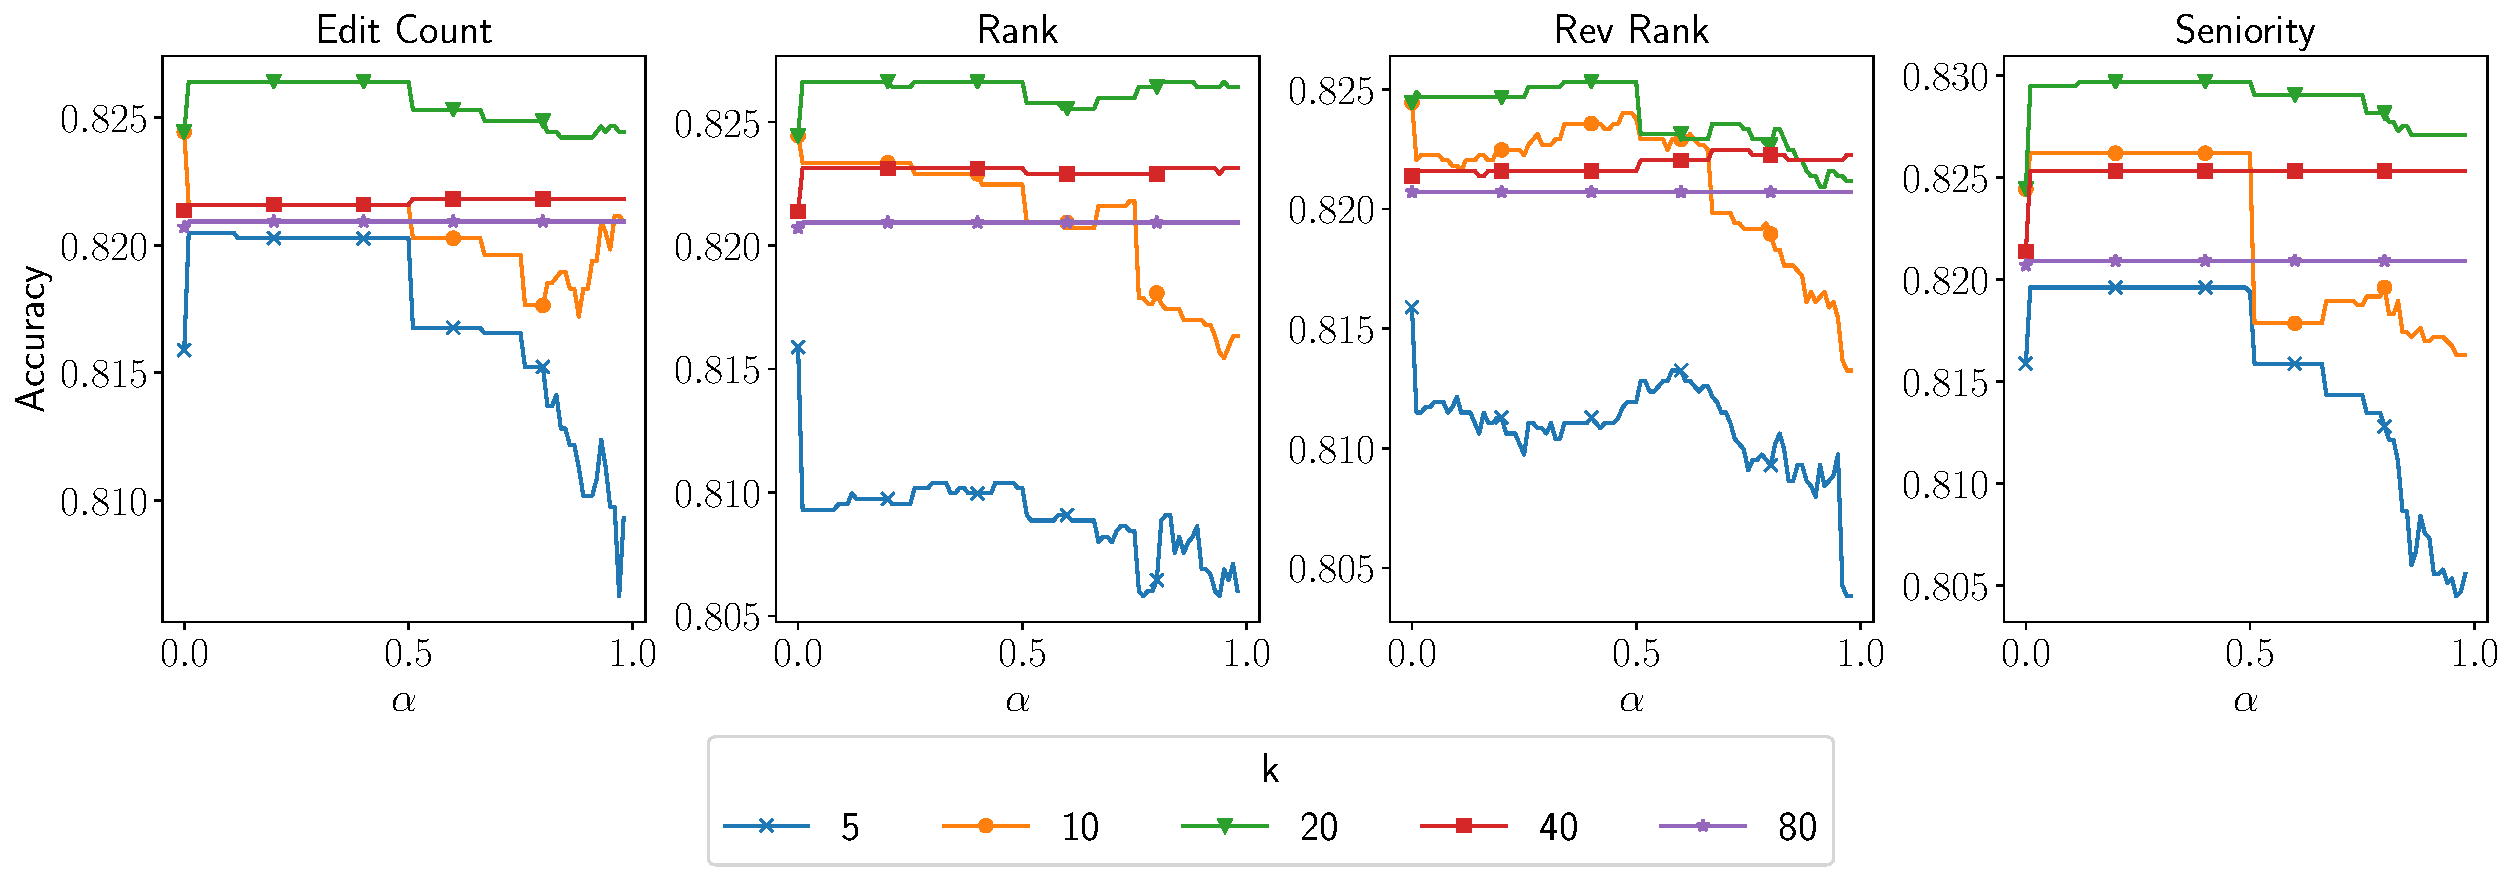
\includegraphics[width=\linewidth]{images/alpha_local.pdf}
    \caption{Effect of $\alpha$ for the Local Tally Viscous Model with different delegation rules and values of $k$}
    \label{fig:local-alpha}
\end{figure*}
\begin{figure*}[t]
    \centering
    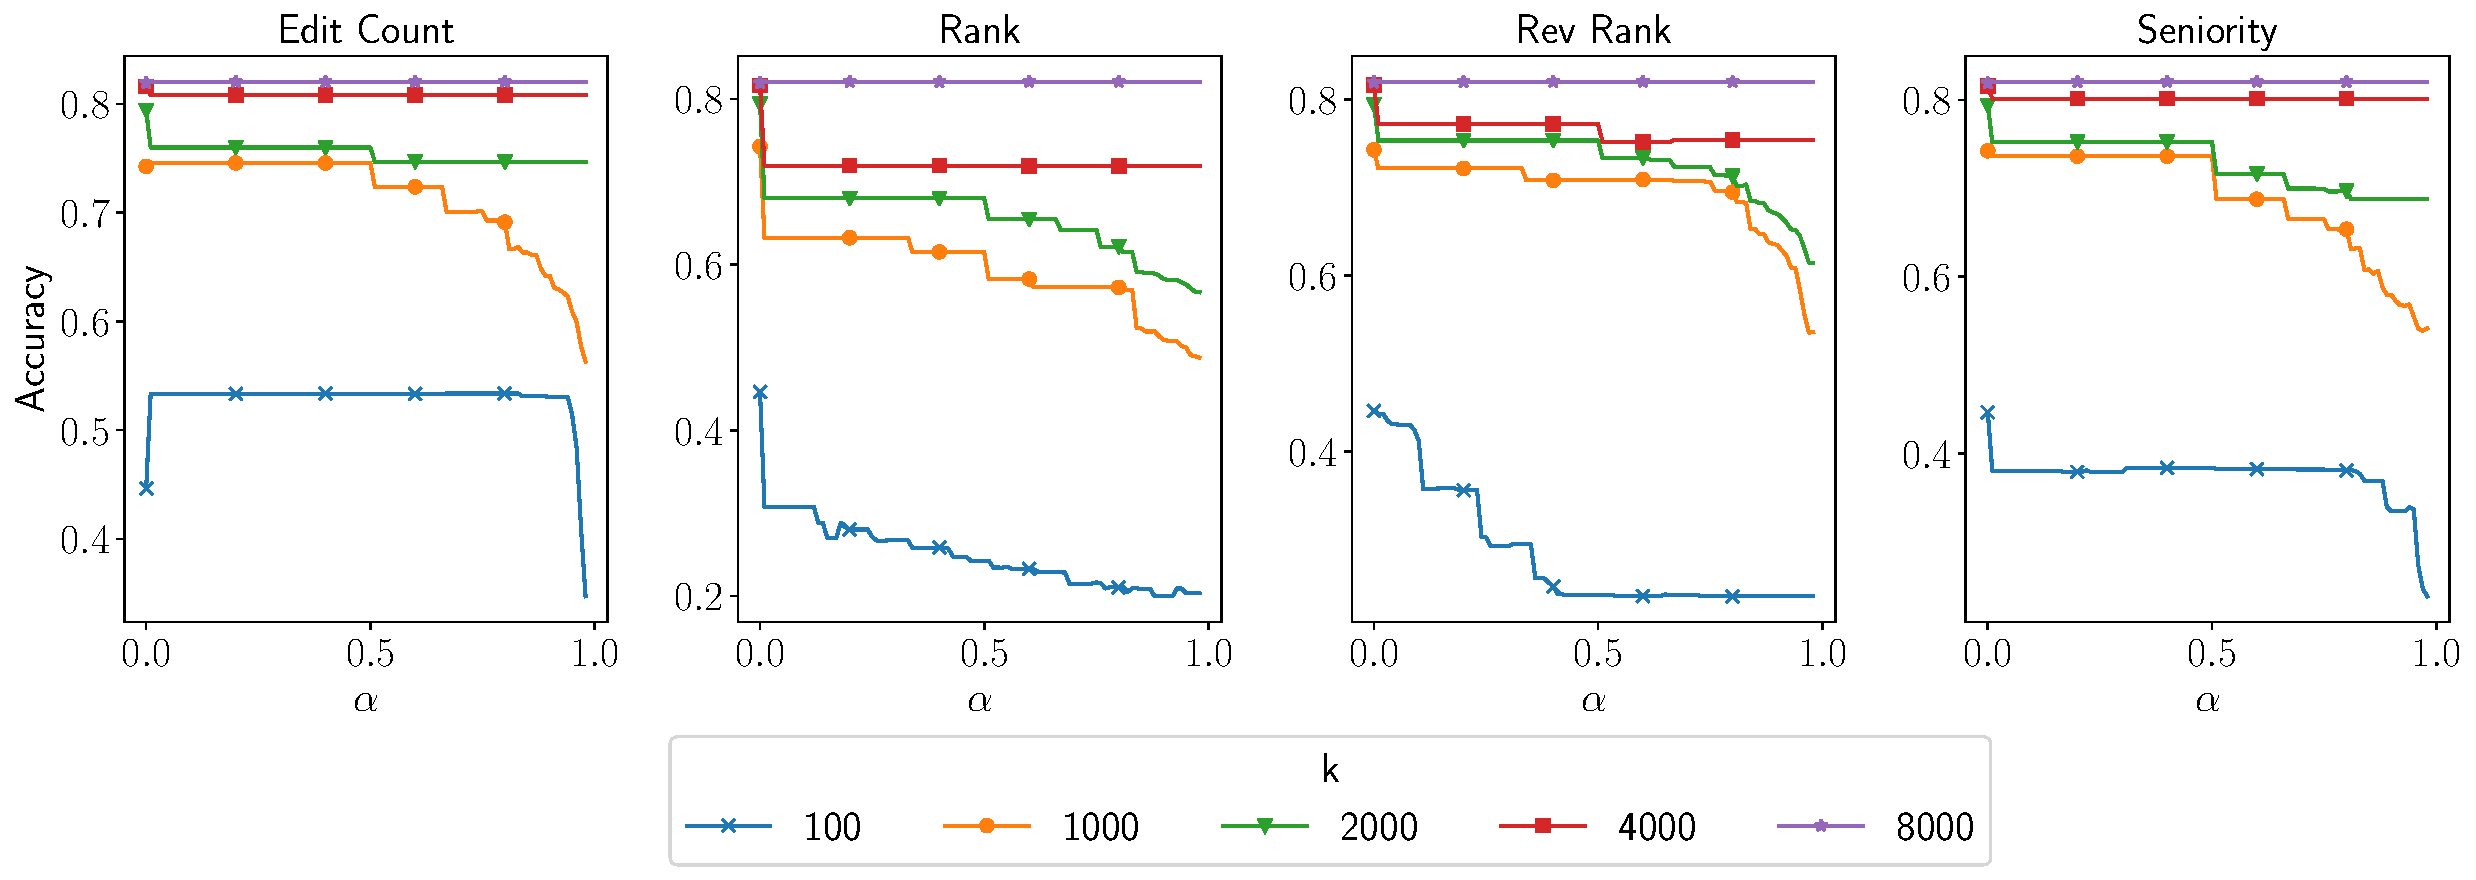
\includegraphics[width=\linewidth]{images/alpha_global.pdf}
    \caption{Effect of $\alpha$ for the Global Tally Viscous Model with different delegation rules and values of $k$}
    \label{fig:local-alpha}
\end{figure*}

\label{sec:results}
We presents the results of the viscous democracy model and analyze the effects of the various parameters on the accuracy of the model.
\smallskip


The main metric we will be using to compare the quality of the Viscous Model is \textbf{accuracy}. The baseline that we will be using to measure the model is a simple tally of all the votes in an RfA election. This compares the most directly with our models as we increase the value of $k$. As we discussed before generally Wikipedia RfA results are positive if there is at least $65\%$ supporting votes. Therefore we filter out elections that have fewer than 10 votes to get a better view of the predictive quality of the model.The baseline model of just tallying the votes gives an accuracy of $\mathbf{82\%}$. 
\smallskip

There are many parameters that have an effect on the predictive accuracy of the model. This means that the effective size of search space is quite large especially as parameters like $\alpha$ have a continuos domain. To narrow the search space as well gather a better understanding of the effects each parameter has on the model we fix all others and take a closer look in the following subsections. Finally we discuss the results of the grid search over the pruned parameter space to find the best performing model.

\subsection{Effect of $\alpha$}
The 
\subsection{Effect of $k$}

\subsection{Grid Search}


The quality of predictions using local or global important editors.